%!TEX root = thesis.tex

\section{Evaluation}
We evaluated the capability and usability of \systemname{} in three lab-based studies.
%, we conducted three user studies to answer questions regarding different authoring aspects:
% (Q1-3): \emph{How well do users understand static motion illustrations? Can users generate step-by-step illustrations with our system?} And \emph{can users refine illustrations with our system?}
%
% Since our motivation is to create illustrations that can be understood and learned,
The first study with 10 participants tested the effectiveness of illustrations generated by \systemname{} (\emph{How well do users understand static motion illustrations?}).
%
The second study with the same participants evaluated the \phaseI{} for recording motion demonstrations (\emph{Can users generate step-by-step illustrations with our system?}).
%
The third study with 4 different participants evaluated the \phaseII{} for editing a pre-captured recording (\emph{Can users refine illustrations with our system?}).
%
%We describe the details of each study with results in the sections below.
Recall that our survey found current methods (using software like Adobe Illustrator) are time intensive, require design expertise, and make iteration difficult.
For these reasons, we did not include a baseline in our evaluations.

% ---------------------------------------------------------------

\subsection{Study 1: Illustration Effectiveness}

We hypothesized that learners can understand and re-perform motions after reviewing step-by-step illustrations generated by \systemname{}.
% \subsubTitleBold{Participants}
To validate, we recruited 10 participants (5 females), aged 18 to 33 years (M=24.3), from a university and an IT company.
%
Six participants had previously created illustrations (from 5 to 50 diagrams, typically using Adobe Illustrator), but none involved body motion. %Four also had experience using 3D modeling software. %, including Blender, Unity, AutoCAD, and SolidWorks.
%
%Among all participants, four were comfortable performing dance moves.
%
% \subsubTitleBold{Experimental Setup}
%In a lab environment,
%
% \subsubTitleBold{Procedure and Tasks}
We first showed the illustrations in Figure~\ref{fig:existing_examples} to introduce the context,
%
then we presented two sets of printed diagrams generated by our the experimenter using our system. There were 16 highlighted joint movements in 8 steps in total (see Figure~\ref{fig:study_review_tasks}).
For each set, participants interpret the illustrations and performed the movements in front of a video camera. %Illustration printouts were placed next to the video camera so that participants did not have to memorize the sequence.
%
% On average, the study lasted 4 minutes; participants practiced one minute and half minute respectively for the two sets prior to recording.

% \subsubTitleBold{Measures}
\subsubTitleBold{Measures and Results}
We coded each joint movement using the video recordings as follows: (M1) the user moved the correct joint; (M2) the start and end positions were approximately correct; % (e.g., moving right hand from lower left to upper right to the body);
 and (M3) the movement was performed correctly (e.g., moving hand straight).
%
Out of 160 re-performed motions across all 10 participants, 85\% motions were completely correct (i.e., M1, M2, M3 all correct). On average, each participant performed 87.2\% of the motions correctly (sd=7\%). No users intentionally moved non-annotated joints.
% All participants successfully performed at least 5 of the 8 steps, with 10 of the 16 joint movements being correct (62.5\%). %For the remaining 6 movements in 3 steps, four were partially correct by 2-4 participants, one had an incorrect start position by 5 participants, and one was missed by 7 participants.
Table~\ref{tab:study1_errors} shows 6 motions that resulted in errors. These motions fall into two classes: temporal sequencing of multiple joints moving in a single step; and cyclic actions (e.g., waving).
%
Some participants could read and re-perform these more complex motions, but there may be limits to what motion diagrams can convey.
%
% We did not code the speed of movements as our illustrations did not convey this element.

% lists systematic errors made by our users and explanations they provided for them. Bi-directional arrows, motions involving independent trajectories of multiple body parts, following complex trajectories, and inferring starting positions from arrows were all sources of errors. We suspect that some of the misinterpretations from our illustrations could be clarified via other visualization styles that \systemname{} is able to generate. We validate this in Study 3.

\begin{table}
  \centering
  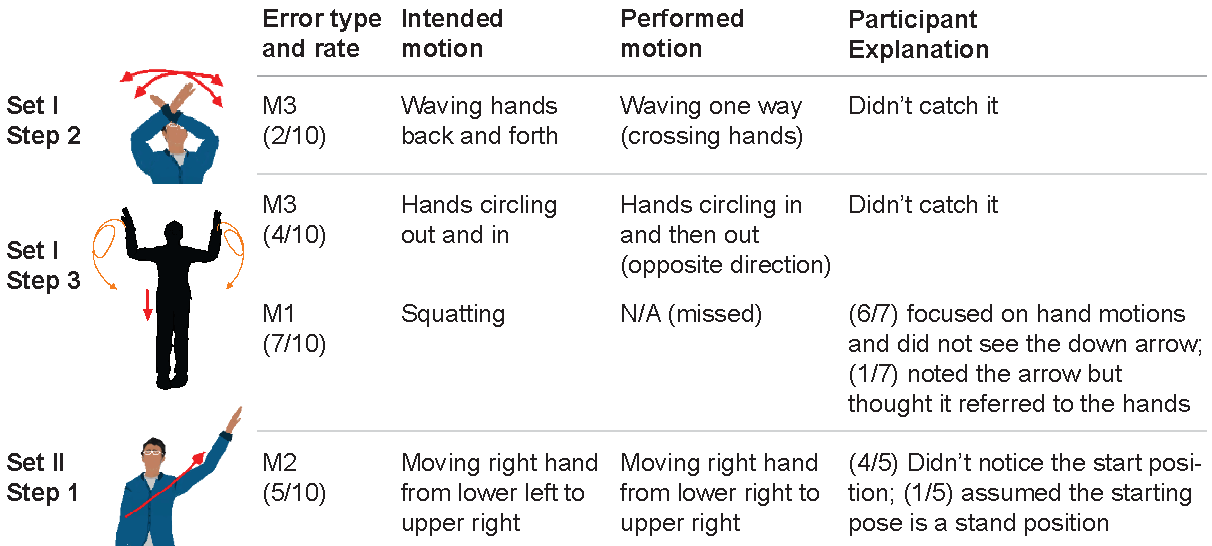
\includegraphics[width=\columnwidth]{\demodraw/fig/study1/study1}
  \caption{Incorrect movements performed by participants in Study 1.}
  \label{tab:study1_errors}
\end{table}

% ---------------------------------------------------------------

\subsection{Study 2: \phaseI{}}

% \subsubTitleBold{Hypothesis}
We hypothesized that amateurs can efficiently create motion illustrations using \systemname{}'s multi-modal \phaseI{}.
%
% \subsubTitleBold{Participants}
Immediately after Study 1, the same 10 participants completed this study (total time was 45 to 60 minutes).
%They were compensated with a \$15 gift card if they completed both studies.

%
% \subsubTitleBold{Procedure and Tasks}
Study 2 began with training where participants were introduced to \systemname{} and shown how to create the second set of illustrations from Study 1.
%The experimenter recorded and reviewed the 4 moves twice.\bjoern{I don't understand what this sentence says - you performed the moves and recorded them into DemoDraw?}
Participants then recorded the same motions and reviewed the results (training was 5 to 10 minutes).
%
Then, four tasks were completed in sequence:
\begin{enumerate}
  \item The experimenter demonstrated 4 moves for a gestural interface with their right hand: waving, circling, a reversed V shape, and right swipe (see Figure \ref{fig:study_authoring_tasks}-1). Participants were asked to record these motions and review the captured results. Once satisfied, they rated the generated illustrations.
  \item Similar to task 1, but with 8 dance moves (see Figure~\ref{fig:study_authoring_tasks}-2).
  \item The experimenter introduced the retake operation and asked participants to choose one step from task 2 to revise. Participants re-performed the motion and reviewed.
  \item Participants were asked to perform any 4 to 8 moves they could imagine and retake them until they were satisfied with the results (within a time limit of 5 minutes).
\end{enumerate}
%The number of attempts were not restricted.
%
% \subsubTitleBold{Experimental Setup}
% The study was conducted in the same space as Study 1.
The system was displayed on a 30-inch monitor (with mouse and keyboard) and the Kinect sensor was placed 3-feet above the floor, capturing 8$\times$8-feet of clean space.

\subsubTitleBold{Measures}
%
In tasks 1 and 2, participants rated each step along five dimensions: (Q1) \iquote{The visualization accurately captured/described my motion}, (Q2) \iquote{The visualization shows all the important joints of movement}, (Q3) \iquote{It shows at least one extraneous joint}, (Q4) \iquote{The key pose was appropriately chosen}, and (Q5) \iquote{This figure needs more (manual) editing before I would share it with others.}
%
The scale for Q1 was a 5-point Likert scale from ``1: Strongly disagree'' to ``5: Strongly agree'' and Q5 was from ``1: Definitely needs edits'' to ``5: Very comfortable to share as is''. The answers for Q2 to Q4 were ``Yes'', ``No'', or ``N/A''.
%
%
%An online questionnaire for overall experiences was provided at the end of the study. Answers to both Likert-scale questions and comments were collected.
Other comments and qualitative feedback were also collected.

\subsection{Study 2 Results}
On average, participants completed task 1 in 5 mins with $\mu=2.3$ takes, task 2 in 10 mins ($\mu=2.8$ takes), task 3 in 3 mins ($\mu=2.3$ takes), and task 4 in 5 mins ($\mu=2$ takes).
% General comments and observations you made about system performance.
Figure~\ref{fig:study_authoring_tasks} and Figure~\ref{fig:open_ended_examples} provide examples of illustrations created by participants. Below we discuss participant feedback on generated illustrations and system design.

\subsubTitleBold{Ratings and Accuracy}
Overall, participants thought the illustrations accurately described their motions (Q1 median ratings of 4.5 for task 1 and 4.88 for task 2).
However, on average participants rated 4 of the 12 steps as requiring further editing to share with others (Q5 median ratings below 3 for both tasks). Figure~\ref{fig:ratings_graphs} shows ratings for each step.
%
Participants commented,
\iquote{This figure represented the overall motion well (...) In particular, it captured all key poses, and the motion lines are easy to follow} (P8),
but also \iquote{the system picked up really small movements in my other joints that were not relevant to the motion I was trying to depict (such as a small motion in my wrist or elbow)} (P1).

\begin{figure}[t]
\centering
$\begin{array}{rl}
    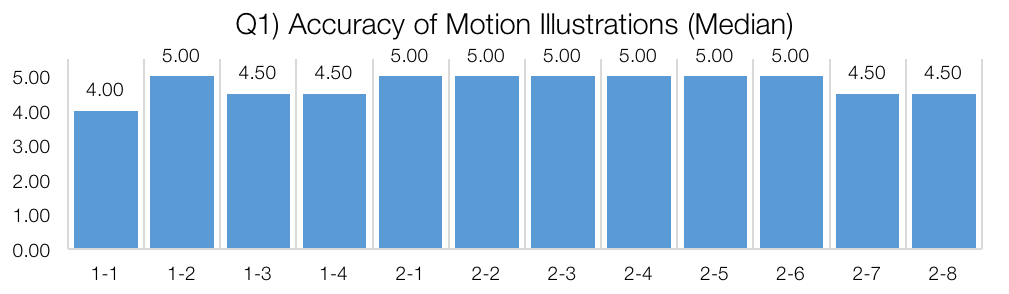
\includegraphics[width=0.6\columnwidth]{\demodraw/fig/study2/q1_accuracy}\\
    \multicolumn{2}{c}{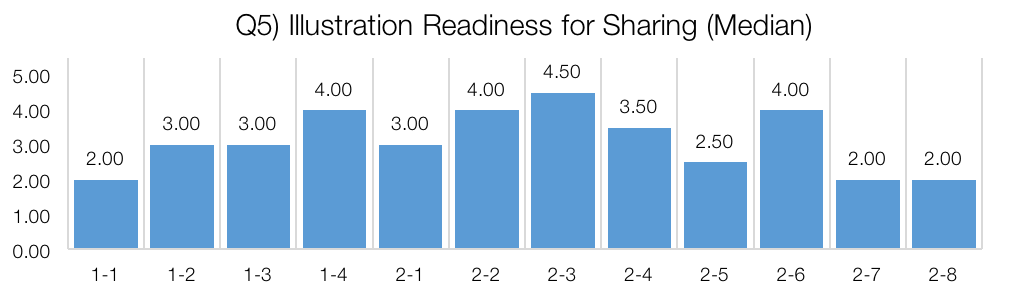
\includegraphics[width=0.6\columnwidth]{\demodraw/fig/study2/q5_editing}}
\end{array}$
\caption{Study 2 median ratings for Q1 and Q5 by illustration step.}
\label{fig:ratings_graphs}
\end{figure}

Across all 120 illustrations created all 10 participants, 99\% showed all the important joints (Q2), and 80\%  precisely selected only the salient joints without extraneous movements (Q3). Participants commented:
%
\iquote{the picture correctly represents my stance and body position. the arrows are easy to see and follow} (P1),
%
\iquote{the lines were very accurate} (P2), and
%
\iquote{the arcs are gorgeous and represent the intention of my motion really well} (P5).
% \iquote{The figure represented the most important poses and movement directions.} (P8)
% \iquote{all of the motions were represented pretty accurately} (P1)

%\subsubTitleBold{Motion Capturing and Analysis}
%Participants were satisfied with our automatic techniques on visualizing their demonstration (M=4.2 and 4.6 for task 1 and 2 respectively in a 5-point Likert scale). They commented:
%\iquote{I'm impressed that the system captured the back and forth of my wave} (P5) and
%\iquote{Swiping motions, making a circle. When it gets the motion, it gets it perfectly} (P7) for task 1.
%Segmentation results were also positive:
%\iquote{Most of the time, the arrows are only attached to key joints that move} (P2).
%
Several participants appreciated how \systemname{} smoothed the motion arrows, especially when their demonstration was not perfect or there was capture noise.
%
%Others noted the advantage of 3D motion data
During the debrief session, participants were shown  illustrations from different  camera viewpoints and several noted the advantage: \iquote{I love the multiple camera angles for the wiggle arm motion I did in step 1} (P9).
% \iquote{I also liked that in most steps the arrows were only on the key motions, and all of the motions had smooth arrows.} (P8)

\subsubTitleBold{Key Pose Selection}
The answers to Q4 showed 94\% of key poses were selected correctly. Example comments include:
%\iquote{It does a great job with the key poses!} (P3),
%\iquote{This figure captured the key poses perfectly} (P8),
%\iquote{All of the key poses in the 8 figures are chosen wisely} (P10),
\iquote{The key poses are very descriptive of the motion} (P2), and
\iquote{The key frames were just right} (P5).

\subsubTitleBold{Authoring Workflow}
Participants found \systemname{} easy to learn (Median 5 out of 5) and easy to create illustrations with (Median 4.5).
\dan{What rankings are these referring to? None of Q1 to Q5 talk about learning, should you be explaining other questions?}
%P9 liked our system as it was \iquote{fast and easy to use; just demonstrate and the motion is captured}, and
%P4 \iquote{was super excited to get great results on my first take.}
%
%We believe that the multi-modal interaction design is suitable for a motion-driven application like \systemname{}.
All participants were able to author and navigate using the speech interface. For example,
\iquote{The voice command allows people be able to control the system remotely. Without the voice capability, the system can be impractical in the single-person use case} (P10).

Participants were especially impressed by how fast authoring could generate a step-by-step diagram:
\iquote{Surprisingly fast to make some really cool full-body motion demonstrations. There is no way I could do this in higher-fidelity than a napkin sketch in the same time} (P5) and
\iquote{the system saves significant amount of time creating illustrations} (P10).
%
We also asked participants to estimate the time required if they were to generate a similar 8-step diagram without using \systemname{}, four participants answered that they would not be able to create them manually, while others responded that it would take 90 to 160 minutes based on each single figure taking 10-20 minutes.
%
%\iquote{Using illustrator alone, I wouldn't be able to create these types of illustrations but using this system I can} (P8),
%\iquote{it was much faster, and you didn't need any photo editing experience to create your own illustrations} (P1), and
%\iquote{Can get a lot of work down in a relatively small amount of time compared to other systems} (P6).
% \iquote{Very quick and efficient. And then can edit post-recording to make it look nice. Can get a lot of work down in a relatively small amount of time compared to other systems.} (P6)

\subsubTitleBold{Improving a Demonstration}
The immediate visual feedback during the capturing phase was effective in helping authors review, adjust, and retake their performances.
P4 explained, \iquote{I learned how to exaggerate the important aspects of motion without being explicitly told to.}
%This was also observed from most participants as they adjusted the motions and re-performed the motions after playing back the illustrations.
In task 3, when we introduced the retaking capability, participants commented that this function would be especially helpful for a long motion sequence. All but one participant chose to retake step 2-7, which involved a holding position with one foot. %Instead of redoing the six steps beforehand, they redid step 2-7 and 2-8 several times (M=2.3 takes).
Three participants later used the same technique for task 4. P8 also noted that it was helpful as \iquote{I could improve this by retaking that step and moving smoothly} when referring to a specific pose they thought needed additional work.
% \iquote{it was fun.} (P9)
% \iquote{So much easier, smaller barrier of entry } (P7)
% \iquote{I like these illustrations because the focus of the diagram is on the motion.} (P8)

% ---------------------------------------------------------------

\subsection{Study 3: \phaseII{} Effectiveness}

To understand how users refine automatically-generated results and generate different visualization styles in \phaseII{}, we conducted an informal study with 4 participants from an IT company (all males, aged 23 to 32 years, M=28).
%
The same apparatus as Study 2 was used.
%and \$15 compensation as Study 2 was used.
% \subsubTitleBold{Procedure and Tasks}
% We provided example illustrations and walked through a warm-up task.
% , including a sign language guide, an airline safety guide, and a Kinect game tutorial
First, experimenters guided participants during a 5-minute training phase
% , which showed a continuous movement of lifting the right hand up and pushing to the right.
 to load one motion recording and create an illustration
% with a thick arrow showing the hand movement
by manipulating a set of visual parameters. %the motion segmentation boundary, selecting joints of interests, line width and color, visual styles, and viewpoints.
%
% This learning phase was 5 minutes on average.
%
% Four tasks were given in sequence:
% To evaluate if our system could support both creating specific illustrations and designing user-generated motions, we designed two parts of a study:
% included two types of tasks: 1) Given an illustration of a motion capture file captured and created by the authors, approximate the illustration with \systemname{}, and 2) given a movement specified by the experimenter in front of the participants, physically record and create an illustration using \systemname{}'s authoring UI.
%
% In tasks 1 and 2,
In the evaluation phase, participants were given two motion recordings, each with three illustrations created using our system. We presented the printed figures one by one and asked them to reproduce them.
% Task 1 showed a motion of two hands waving in opposite directions, which involved two joints and change of default arrow style. Task 2 showed a motion that a person squat down after circling two hands, which involved multiple joints (two with relative positions) and change of camera viewpoint.
%
% In tasks 3 and 4,
Participants then used \systemname{} to physically perform and record two specific motions given by the experimenter,
% Experimenters helped hit the record button when they indicated that they were ready.
and create illustrations to best convey each motion.
% They were free to use any skills they had learned without time limitation. % from the previous tasks
%
% Finally, an online questionnaire was provided.

\subsubTitleBold{Results}
% All the participants successfully completed the tasks and created illustrations. (see Figure~\ref{fig:study3_results} for selected examples).
%
%Similar to Study 2, participants found it easy to learn (M=4.25 out of 5) and create a motion illustration (M=4.5) using \systemname{}. P1 commented that it was \iquote{Super easy to use and create different illustration styles quickly}, and P3 thought, \iquote{the fact that you can change up the colors and characters is a cool bonus!}
%
%As this study provided more versatile visualization techniques,
Participants actively experimented with visual parameters and styles provided by the \phaseII{}, especially when creating stroboscopic effects. For example: number of intermediate frames and offset, dragging to reposition the arrows, and arrow color and width.
%
In addition, participants formed strong preferences for styles once given these visualization options. For example, P4 said the stroboscopic effect in task 3 \iquote{is exactly what I looked for -- It clearly conveys the start and end poses.} P2 preferred the cartoon renderer over the silhouette since \iquote{this character looks just like me!}
%
All said they could not create similar illustrations without \systemname{} (Median 2 out of a 5-point Likert scale).
%
\dan{this is a bit confusing since I don't know what the question or the scale was.}
This indicates  detailed editing with the \phaseII{} was effective and expressive for various motion types.

\begin{figure}[t]
  \centering
  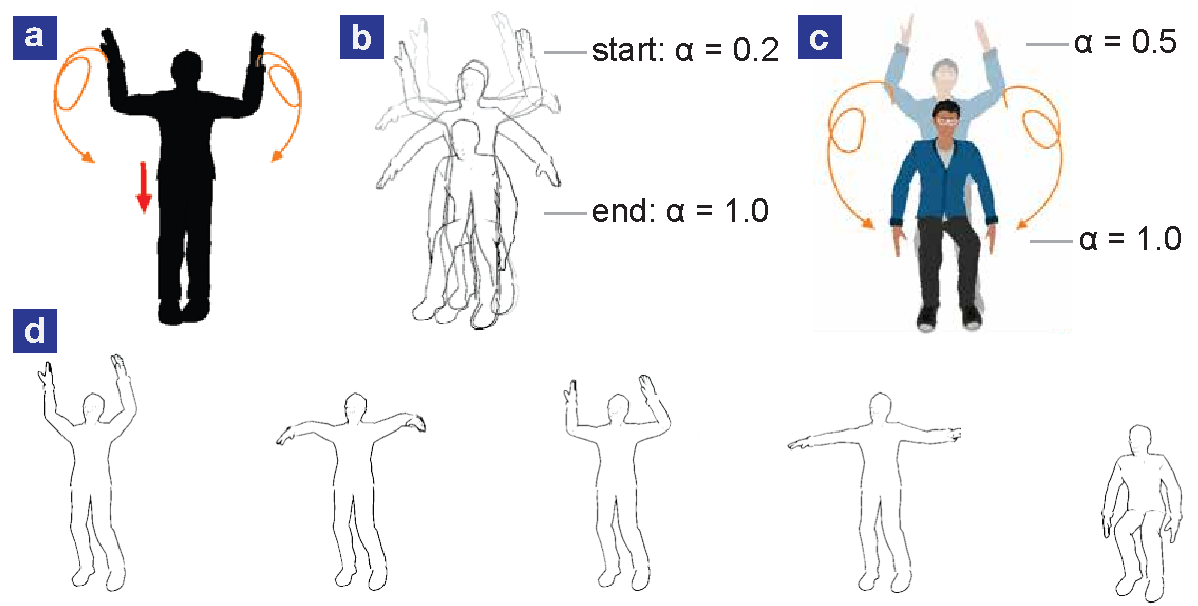
\includegraphics[width=0.8\columnwidth]{\demodraw/fig/study3/study3_effects}
  \caption{Different illustration effects conveying the same motion recording using \systemname{}'s \phaseII{}: a and c are created by the authors of this work and a was used in Study 1; b by Study 3-P1 using 4 intermediate frames with zero offset; d by Study 3-P2 using 5 frames, positioned as a sequence.}
  \label{fig:study3_effects}
\end{figure}

\subsection {Discussion}

Participants were clearly excited about the overall experience using both the \phaseI{} and the \phaseII{}.
%Comments we received included, \systemname{} is a \iquote{REALLY COOL SYSTEM} (Study 2-P7), \iquote{Seriously, the poses look really cool! I want the last one to be my profile picture} (Study 2-P3), and \iquote{Great idea overall, this will save lots of time for whoever is designing these artworks :)} (Study 3-P3).
%
Some explicitly pointed out their enjoyment:
% \iquote{Overall, it's a lot of fun, and I can see it being really helpful for anybody trying to explain motion} (P3),
\iquote{it accurately captures how much fun I had making it. :)} (Study 2-P9), and
\iquote{For professional artists, the system not only increases their productivity, but also brings joy and fun to this kind of tasks} (Study 2-P10).
%
Participant feedback suggests motion illustrations generated by \systemname{} are expressive enough to depict their demonstrations. Our multi-modal interface with motion analysis and rendering algorithms enabled users to quickly create step-by-step diagrams.
\dan{I moved the ``no baseline of Illustrator'' argument back to the study section.}

\bjoern{I'm not really sold on the rest of this section - some of it feels too low level. Not sure what to do here.}

\dan{One of the main things to discuss (with some convincing arguments based on specific results from the three studies) is whether we achieved our primary goals and answered research questions:
1) the system makes good looking diagrams quickly; (reference back to how long current methods take)
2) the iterative/interactive demonstration style is key to this success. (reference back to how non-iterative current methods are) }

\dan{Another discussion topic is the implications of this system. If the iterative/interactive demonstration style worked here, would it be better in other demonstration systems too? What should interaction designers learn from this at a level above the specific motion illustration task?}

\subsubTitleBold{Support of Various Styles}
In Study 1, motion arrows successfully conveyed the majority of movements. When arrows alone are not adequate, stroboscopic could be combined to clarify details in the start, intermediate, and end poses. For example, the simultaneous hand movements and squatting action of Step 3 in Study 1 are difficult to convey using only arrows (see Table~\ref{tab:study1_errors}), but Study 3 participants chose a stroboscopic effect to convey the same motion (see Figure~\ref{fig:study3_effects}).
%
These findings align with existing instructional design principles~\cite{mijksenaar1999open}, which suggest designers combine illustration styles based on the context. An authoring interface (like \phaseII{} in our system) must make it easy to adjust styles and parameters within a style (i.e., an outline figure with motion arrows).

\subsubTitleBold{Iterative Creation Process}
Our studies verified our earlier findings that creating motion illustrations is an iterative procedure, where (re-)performing, reviewing, and refining are necessary components (see Figure~\ref{fig:designspace}).
In Study 2, we observed how retaking a partial demonstration could be useful for long step-by-step motion sequences; Study 3 suggested that once moving into a refinement phase, authors focused on detailed adjustments of captured movements. Ensuring a high-level review of capturing results during demonstrations is therefore important.

\subsubTitleBold{Animation vs. Illustration}
As \systemname{} captures the continuous motion sequence in 3D from a demonstrator, our system also generates animations showing the dynamic movements.
%
In the warm-up task of Study 2 that captured the second motion set in Study 1, some participants explained that the playback animation of the recording clarified the motion where they incorrectly interpreted the start position.
%
We propose that as motion arrows can efficiently and effectively express most of the motions, a mixed-media version can be created, where viewers can selectively review part of a static diagram with in-place animation playback. Such format has been shown to be useful for clarifying step-by-step instructions~\cite{Chi:2012:MAG:2380116.2380130}. In addition, the 3D reconstruction also makes it possible to review motions from different viewing angles.
%
All in all, our technology enables both instructors and viewers to interactively create and review motion illustrations in multiple ways.

\subsubTitleBold{Design Implications}
In this work, we focus on body motion diagrams.
% , which are an important class of visualizations for a variety of domains including sports, dance, and full-body/gestural interfaces.
More broadly, we believe our work also provides findings and techniques that apply to other demonstration-based systems. First, our multi-modal interface enables authors to perform critical tasks without leaving the demonstration context. Second, separating demonstration capture from detailed refinement allows users to focus solely on performance at demonstration-time while preserving the ability to fine-tune results later on. Third, clear, real-time illustration previews of performed motions enable fast iteration at demonstration.
% - Observations about what types of human motions can be concisely conveyed via simple static diagrams.
